\documentclass{article}
\usepackage{tikz}
\usetikzlibrary{shapes.geometric, arrows}

\tikzstyle{startstop} = [rectangle, rounded corners, minimum width=2cm, minimum height=1cm, text centered, draw=black, inner sep=2pt]
\tikzstyle{process} = [rectangle, minimum width=2.5cm, minimum height=1cm, text centered, draw=black, inner sep=2pt]
\tikzstyle{arrow} = [thick,->,>=stealth]

\begin{document}
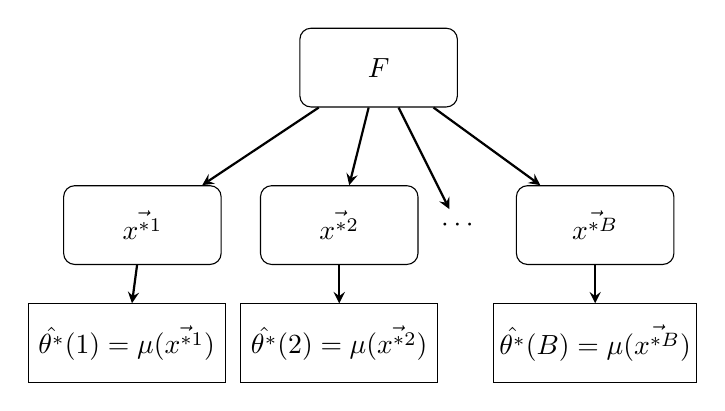
\begin{tikzpicture}[node distance=1.5cm]

% Root node
\node (F) [startstop] {$F$};

% First row nodes
\node (x1) [startstop, below of=F, xshift=-3cm, yshift=-0.5cm] {$\vec{x^{*1}}$};
\node (x2) [startstop, below of=F, xshift=-0.5cm, yshift=-0.5cm] {$\vec{x^{*2}}$};
\node (dots) [text centered, below of=F, xshift=1cm, yshift=-0.5cm] {$\cdots$};
\node (xB) [startstop, below of=F, xshift=2.75cm, yshift=-0.5cm] {$\vec{x^{*B}}$};

% Second row nodes
\node (theta1) [process, xshift=-0.2cm, below of=x1] {$\hat{\theta^*}(1) = \mu(\vec{x^{*1}})$};
\node (theta2) [process, below of=x2] {$\hat{\theta^*}(2) = \mu(\vec{x^{*2}})$};
\node (thetaB) [process, below of=xB] {$\hat{\theta^*}(B) = \mu(\vec{x^{*B}})$};

% Drawing arrows
\draw [arrow] (F) -- (x1);
\draw [arrow] (F) -- (x2);
\draw [arrow] (F) -- (dots);
\draw [arrow] (F) -- (xB);
\draw [arrow] (x1) -- (theta1);
\draw [arrow] (x2) -- (theta2);
\draw [arrow] (xB) -- (thetaB);

\end{tikzpicture}

\end{document}
